\documentclass[preprint]{sigplanconf} % <<<

\usepackage{amsmath}
\usepackage{amssymb}
\usepackage{amsthm}
\usepackage{graphics}
\usepackage[latin1]{inputenc}
\usepackage{microtype}  % do not remove
\usepackage{pygmentize}
\usepackage{rgalg}
\usepackage{tikz}
\usepackage{xcolor}

\usepackage[colorlinks]{hyperref}

\RecustomVerbatimEnvironment{Verbatim}{BVerbatim}{}
\definecolor{darkblue}{rgb}{0,0,0.4}
\definecolor{verylightgray}{rgb}{0.9,0.9,0.9}
% comment the next line for printing
\hypersetup{colorlinks,linkcolor=darkblue,citecolor=darkblue,urlcolor=darkblue}
\hypersetup{
  pdftitle={A Language for Specifying Safety Temporal Properties of Object-Oriented Programs},
  pdfauthor={Dino Distefano and Radu Grigore and Rasmus Lerchedahl Petersen}}

\titlebanner{DRAFT}
\title{A Language for Specifying Safety Temporal Properties of Object-Oriented Programs}
\authorinfo{Dino Distefano \and Radu Grigore \and Rasmus Lerchedahl Petersen}{Queen Mary, University of London}{{\rm\{}ddino,rgrig,rusmus{\rm\}}@eecs.qmul.ac.uk}

\newcommand{\dinocomment}[1]{
\begin{center}
\fbox{
\begin{minipage}{3.0in}
{\bf Dino's comment:} {\it #1}
\end{minipage}}
\end{center}}

\newcommand{\note}[2]{\textcolor{gray}{[\textcolor{red}{#1}: #2]}}
\newcommand{\rg}[1]{\note{rg}{#1}}

\newcommand{\N}{\ensuremath{\mathbb{N}}}
\newcommand{\eval}[1]{[[#1]]}
\newcommand{\pmap}{\rightharpoonup}
\newcommand{\set}[1]{\ensuremath{\mathsf{#1}}}
\newcommand{\verbline}[2][]{\[\text{\Verb@#2@}#1\]}

\theoremstyle{definition}
\newtheorem{example}{Example}

\overfullrule=5pt
\showboxdepth=10
\showboxbreadth=30
% >>>
\begin{document}
\maketitle

\begin{abstract} % <<<
In this paper we present a new specification language for temporal safety properties aimed at object-oriented languages.
The language is expressive enough to represent relationships between objects and it is designed with the goal of performing dynamic and static analysis of object-oriented software.
\end{abstract}
\category{D.2.1}{Software Engineering}{Requirements/Specifications}
\terms Languages, Verification
\keywords Safety, Temporal Properties, Object-Oriented

% >>>
\section{Introduction} % <<<
One popular class of properties addressed by many techniques in program verification is to check whether a program satisfies some specified safety property.  
Violations of this class of properties may lead to unexpected run-time errors.

Many safety properties can be expressed using the framework of {\em typestate}~\cite{strom1986} which uses finite state automata for specifying conformance or violation w.r.t. a temporal safety property.

The long term aim of our project is the automatic verification of typestate properties of Java programs of realistic size.  
The properties should be given by the user; they should not be hard-coded.
In order to achive our goal we would need
\begin{itemize}
\item A language for specifying temporal safety properties;
\item An automatic tool that can verify the properties in the language
  against Java programs.
\end{itemize}
This paper addresses the first point by introducing {\em TPL} (Temporal Property Language). 
\dinocomment{Come up with a better name or drop it!}
It has the following characteristics:
\begin{itemize}
\item It is designed for OOP. 
And since object-oriented languages like Java make heavy use of the heap, we have designed our language based on separation logic~\cite{reynolds2002} a formalist known to be effective and concise in specifying heap related properties.
\item It allows very high-level intuitive specifications which are given with an special form of automata.
\item It is designed to be used to do program analysis (both static and dynamic).
\end{itemize}  
In this paper we introduce the language and its formal semantics. 
Moreover we show how this can be used for doing dynamic checking of its properties using a simple object-based language.

% contributions
% - language for temporal properties
% - keep references (object) relationship
% - designed for oop
% - designed for doing analysis (dyn/stat)
% - High-level/simple
% Safety (obiquitus)

The paper is organized as follows. In Section~\ref{sec:example} we start with a motivating example. 
Section~\ref{sec:syntax} gives the syntax of TPL and in Section~\ref{sec:semantics} introduces its semantics. 
Section~\ref{sec:testing} describes the use of TPL for run-time checking of safety properties. 
Section~\ref{sec:related} discusses related work and our future plans. 
Finally, Section~\ref{sec:conclusions} conclude the paper.
% >>>
\section{Example}\label{sec:example} % <<<

\rg{I am heavily editing this section, much text is crap now.}

The last statement in \autoref{fig:running.java} throws an exception.
There are two iterators on the same collection, one of them modifies the collection, and this invalidates the other iterator.
The automaton in \autoref{fig:running.property} formally captures the disallowed API usage.
The automaton is given essentially as a list of labeled transitions.
Each label is a statement pattern.
\autoref{fig:running.drawing} shows the same automaton in a graphical form.

\autoref{fig:running.steps} shows how a particular execution of the program drives the automaton.
The automaton is nondeterministic so it has a \emph{set} of active states.
Initially, only the state $(\mathit{start},[])$ is active.
The outgoing transition of vertex \textit{start} is labeled by \[I:=C.\mathtt{iterator}()\] and the statement about to be executed is \verbline[.]{i = c.\PY{n+na}{iterator}()}
To see if the pattern matches the statement we first look at the method.
For simplicity, we identify Java methods by their fully qualified names and their arities.
In this case, the method that is invoked is \verbline[.]{java.util.ArrayList.iterator<1>}
The \texttt{using prefix} directives say that the string \texttt{iterator} is a shorthand for one of two method names.
The pattern matches the methods
\begin{align*}
&\text{\Verb@java.util.Collection.iterator<1>@} \\
&\text{\Verb@java.util.Iterator.iterator<1>@}
\end{align*}
and all the methods that override them.
In this case, the \textit{iterator} method in \textit{ArrayList} overrides the one in \textit{Collection} so we have a match.
Next, we look at the patterns $I$~and~$C$.
By convention, patterns starting with an uppercase letter match any value.
In this case, they match the values held by the program variable $i$~and~$c$.
At this point, all conditions are met to perform the transition from \textit{start} to \textit{gotOne}.
Performing a transition involves remembering the values on which the uppercase patterns matched.
For concreteness, let us assume that the program variables $c$~and~$i$ hold the values $1$~and~$2$.
Then, performing the first transition stores the values $1$~and~$2$ into the \emph{automaton variables} $c$~and~$i$.
The automaton variables live in a different name-space from program variables.
In this case we use the same names for automaton variables as for program variables purely as a mnemonic device---there is no semantics to it.
The end result of performing the transition from \textit{start} to \textit{gotOne} is that the state \[(\mathit{gotOne},[c:1,i:2])\] is activated.
Usually, the source of a transition would not be active anymore.
In this case, the state $(\mathit{state},[])$ remains active because it is a special state that is always active.
Conceptually, the vertex \textit{start} has a loop on it that always matches.

For the second step we need to consider the two active states in turn.
For $(\mathit{start},[])$ exactly the same reasoning holds and the result is that \[(\mathit{gotOne},[c:1,i:3])\] is active after the second step.
Note that now the automaton variable~$i$ remembers the value of the program variable~$j$.
For \[\mathit{gotOne},[c:1,i:2])\] we look at the transition outgoing from vertex \textit{gotOne}.
It has the label \[J:=c.\mathtt{iterator}();\]
the statement to be executed is \verbline[.]{j = c.\PY{n+na}{iterator}()}
The method and the uppercase pattern~$J$ match in the same way as before.
The lowercase pattern $c$ matches only the value that is held by the automaton variable~$c$.
In summary, uppercase patterns write to the automaton memory, and lowercase patterns read from the automaton memory and act as a guard on the transition.
In this case, the transition $\mathit{gotOne}\to\mathit{gotTwo}$ is performed because the program variable~$c$ still refers to the same collection it did when the transition $\mathit{start}\to\mathit{gotOne}$ was performed.

In the third step, no transition is performed and the same states remain active.
None of the outgoing transitions of \textit{start}, \textit{gotOne}, and \textit{gotTwo} match the method \textit{next}.

In the fourth step, the transition $\mathit{gotTwo}\to\mathit{jInvalid}$ is performed for the state corresponding to the vertex \textit{gotTwo}.
The pattern $i.\mathtt{remove}()$ does not have a left-hand side, which simply means that the returned value does not matter.
The states corresponding to vertices \textit{start} and \textit{gotOne} remain unchanged, because their outgoing transitions do not match.

For the fifth and final step, one of the active states is \[(\mathit{jInvalid},[c:1,i:2,j:3]),\] the label on its outgoing transition is \[\mathtt{call}\;j.{*}(),\] and the statement to be executed is \verbline[.]{j.\PY{n+na}{next}()}
The pattern has two distinguishing features, the~$*$ as a method name and the tag \texttt{call}.
Let us discuss first the method name.

\rg{TODO: continue here}


The problem is subtle and appears in practice from time to time.
It is clearly a temporal property (an iterator cannot be used \emph{after} another iterator modifies the collection) and it involves multiple objects (two iterators and one collection).
\autoref{fig:running.property} 


%\autoref{fig:running.java} shows a program that throws \Verb+ConcurrentModificationException+.

X illustrates a subtle temporal property, which is well-known to Java programmers.

The program in~X fails with an exception.
It is usually illegal to modify the underlying collection while iterating.
A collection may be modified through its methods or through the \textit{remove} method of one of its iterators.
The iterator that modifies the collection remains valid; the others must not be used anymore.
We express this last property formally using the following automaton.

X shows a drawing of~TODO.
Properties are structured as labeled digraphs.
The first column lists the arcs;
the second column lists the corresponding arc labels.
The labels look like simple statements in a programming language.
They are in fact statement patterns.
The first label, $I:=C.\mathit{iterator}()$, matches all calls to a method called \textit{iterator}.
The patterns $I$~and~$C$ match any two values and record them in two automaton variables, $i$~and~$c$.
The second label, $J:=c.\mathit{iterator}()$, uses a lowercase~$c$.
Unlike the pattern~$C$, the pattern~$c$ only matches values equal the value of the automaton variable~$c$.
The automaton variables $i$,~$j$, and~$c$ live in a distinct name-space.
The fact that the code in X uses the same names is irrelevant.
The automaton is non-deterministic and it is driven by executions of the program.
Let us assume that the values taken by the \emph{program} variables $c$,~$i$, and~$j$ are, respectively, $1$,~$2$, and~$3$.
Then the parallel execution of the program with the automaton proceeds as follows.

\begin{figure}
\begin{Verbatim}[commandchars=\\\{\}]
\PY{k+kn}{import} \PY{n+nn}{java.util.*}\PY{o}{;}
\PY{k+kd}{public} \PY{k+kd}{class} \PY{n+nc}{IncorrectIteratorUse} \PY{o}{\PYZob{}}
  \PY{k+kd}{public} \PY{k+kd}{static} \PY{k+kt}{void} \PY{n+nf}{main}\PY{o}{(}\PY{n}{String}\PY{o}{[}\PY{o}{]} \PY{n}{args}\PY{o}{)} \PY{o}{\PYZob{}}
    \PY{n}{List}\PY{o}{<}\PY{n}{Integer}\PY{o}{>} \PY{n}{c} \PY{o}{=} \PY{k}{new} \PY{n}{ArrayList}\PY{o}{<}\PY{n}{Integer}\PY{o}{>}\PY{o}{(}\PY{o}{)}\PY{o}{;}
    \PY{n}{c}\PY{o}{.}\PY{n+na}{add}\PY{o}{(}\PY{l+m+mi}{1}\PY{o}{)}\PY{o}{;} \PY{n}{c}\PY{o}{.}\PY{n+na}{add}\PY{o}{(}\PY{l+m+mi}{2}\PY{o}{)}\PY{o}{;}
    \PY{n}{Iterator}\PY{o}{<}\PY{n}{Integer}\PY{o}{>} \PY{n}{i} \PY{o}{=} \PY{n}{c}\PY{o}{.}\PY{n+na}{iterator}\PY{o}{(}\PY{o}{)}\PY{o}{;}
    \PY{n}{Iterator}\PY{o}{<}\PY{n}{Integer}\PY{o}{>} \PY{n}{j} \PY{o}{=} \PY{n}{c}\PY{o}{.}\PY{n+na}{iterator}\PY{o}{(}\PY{o}{)}\PY{o}{;}
    \PY{n}{i}\PY{o}{.}\PY{n+na}{next}\PY{o}{(}\PY{o}{)}\PY{o}{;} \PY{n}{i}\PY{o}{.}\PY{n+na}{remove}\PY{o}{(}\PY{o}{)}\PY{o}{;} \PY{n}{j}\PY{o}{.}\PY{n+na}{next}\PY{o}{(}\PY{o}{)}\PY{o}{;}
  \PY{o}{\PYZcb{}}
\PY{o}{\PYZcb{}}
\end{Verbatim}

\caption{Running example: Java code}
\label{fig:running.java}
\end{figure}
\begin{figure}
\begin{Verbatim}
property "collection was modified by iterator"
  using prefix java.util.Collection
  using prefix java.util.Iterator
  start -> gotOne:    I := C.iterator()
  gotOne -> gotTwo:   J := c.iterator()
  gotTwo -> jInvalid: i.remove()
  gotTwo -> iInvalid: j.remove()
  jInvalid -> error:  call j.*()
  iInvalid -> error:  call i.*()
\end{Verbatim}
\caption{Running example: Safety property}
\label{fig:running.property}
\end{figure}
\begin{figure}
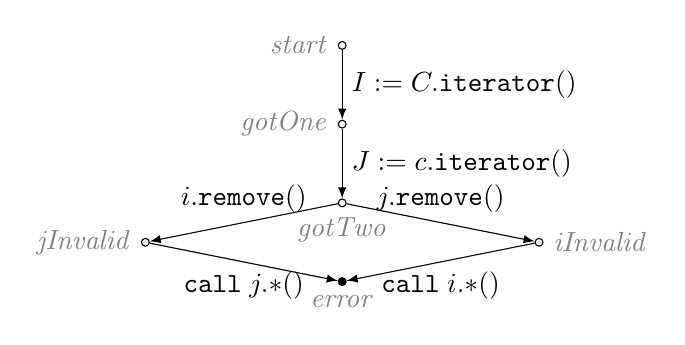
\begin{tikzpicture}[xscale=2.5]
  \tikzset{vertex/.style={draw,circle,inner sep=1pt}}
  \tikzset{transition/.style={->,>=latex}}
  \tikzset{every label/.style={gray}}
  \node[vertex] (start) at (0,0) [label=left:\textit{start}] {};
  \node[vertex] (gotOne) at (0,-1) [label=left:\textit{gotOne}] {};
  \node[vertex] (gotTwo) at (0,-2) [label=below:\textit{gotTwo}] {};
  \node[vertex] (iInvalid) at (1,-2.5) [label=right:\textit{iInvalid}] {};
  \node[vertex] (jInvalid) at (-1,-2.5) [label=left:\textit{jInvalid}] {};
  \node[vertex,fill] (error) at (0,-3) [label=below:\textit{error}] {};
  \draw[transition] (start)--node[right]{$I:=C.\mathtt{iterator}()$} (gotOne);
  \draw[transition] (gotOne)--node[right]{$J:=c.\mathtt{iterator}()$} (gotTwo);
  \draw[transition] (gotTwo) -- node[above]{$j.\mathtt{remove}()$} (iInvalid);
  \draw[transition] (gotTwo)--node[above]{$i.\mathtt{remove}()$} (jInvalid);
  \draw[transition] (iInvalid)--node[below]{$\mathtt{call}\;i.{*}()$} (error);
  \draw[transition] (jInvalid)--node[below]{$\mathtt{call}\;j.{*}()$} (error);
\end{tikzpicture}
\caption{Running example: Drawing of safety property}
\label{fig:running.drawing}
\end{figure}
\begin{figure}
\begin{align*}
&\{(\mathit{start}, [])\} \\
&\text{\Verb+\PY{n}{Iterator}\PY{o}{<}\PY{n}{Integer}\PY{o}{>} \PY{n}{i} \PY{o}{=} \PY{n}{c}\PY{o}{.}\PY{n+na}{iterator}\PY{o}{(}\PY{o}{)}\PY{o}{;}+} \\
&\text{assume $c$ holds $1$, and $i$ holds $2$ } \\
&\{(\mathit{start},[]), (\mathit{gotOne},[c:1, i:2])\} \\
&\text{\Verb+\PY{n}{Iterator}\PY{o}{<}\PY{n}{Integer}\PY{o}{>} \PY{n}{j} \PY{o}{=} \PY{n}{c}\PY{o}{.}\PY{n+na}{iterator}\PY{o}{(}\PY{o}{)}\PY{o}{;}+}\\
&\text{assume $j$ holds $3$} \\
&\{(\mathit{start},[]), (\mathit{gotOne},[c:1,i:3]),(\mathit{gotTwo},[c:1,i:2,j:3])\} \\
&\text{\Verb+\PY{n}{i}\PY{o}{.}\PY{n+na}{next}\PY{o}{(}\PY{o}{)}\PY{o}{;}+} \\
&\{(\mathit{start},[]), (\mathit{gotOne},[c:1,i:3]),(\mathit{gotTwo},[c:1,i:2,j:3])\}\\
&\text{\Verb+\PY{n}{i}\PY{o}{.}\PY{n+na}{remove}\PY{o}{(}\PY{o}{)}\PY{o}{;}+} \\
&\{(\mathit{start},[]), (\mathit{gotOne},[c:1,i:3]),(\mathit{jInvalid},[c:1,i:2,j:3])\} \\
&\text{\Verb+\PY{n}{j}\PY{o}{.}\PY{n+na}{next}\PY{o}{(}\PY{o}{)}\PY{o}{;}+}\\
&\{(\mathit{start},[]), (\mathit{gotOne},[c:1,i:3]), (\mathit{error},[c:1,i:2,j:3])\}
\end{align*}
\caption{Running example: Step by step}
\label{fig:running.steps}
\end{figure}

% >>>
\section{Syntax}\label{sec:syntax} % <<<

\rg{TODO: Present desugarings---things like methods names, going from patterns to guards and actions.}

% >>>
\section{Semantics}\label{sec:semantics} % <<<

A program's semantics is a set of event traces;
an automaton's semantics is also a set of event traces.
A program \emph{violates} a property when their sets intersect.
Both the program and the automaton are nondeterministic.
\dinocomment{So we only want to use the automata to specify bad behaviour? How about good behaviour?}

\subsection{Automaton} % <<<

Each event has a tag and carries an array of values.
\begin{align}
\set{Event}&=\bigcup_{n\in\N}\set{Tag}_n\times(n\to\set{Value})
\end{align}
(As usual, $n=\{0,1,\ldots,n-1\}$.)
The content of the undefined sets (such as \set{Value}) is not important.
We assume that these basic sets are disjoint.
Traces are finite.
\begin{align}
\set{Trace}=\bigcup_{n\in\N} n\to\set{Event}
\end{align}
Intuitively, the program outputs a trace that drives the automaton.

The automaton is defined on top of a finite multi-graph.
The automaton is an array of transitions.
Each transition has an edge and an array of labels.
Each edge has a source vertex and a target vertex.
Each label is a (guard, action) pair.
There are at least two vertices.
\begin{align}
\set{Automaton} &= \bigcup_{n\in\N} n \to \set{Transition} \\
\set{Transition} &= \set{Edge}\times \bigcup_{n\in\N} n\to\set{Label} \\
\set{Edge}&=\set{Vertex}\times\set{Vertex} \\
\set{Label}&=\set{Guard}\times\set{Action} \\
\{\mathtt{start},\mathtt{error}\}&\subseteq\set{Vertex}
\end{align}
The deterministic state contains a store of values.
\dinocomment{this deterministic state seems to come out of the blue.}
A store is a finite partial map from automaton variables to values.
We also define an automaton deterministic execution state, which includes the input to be processed.
\begin{align}
\set{Store}&=\set{Variable}\pmap\set{Value} \\
\set{AState}&=\set{Vertex}\times\set{Store} \\
\set{EAState}&=\set{AState}\times\set{Trace}
\end{align}
Guards compare the values in an event with those in a store.
Actions modify the store, using values from an event.
\begin{align}
\set{Guard}&=\set{Event}\to\set{Store}\to2 \\
\set{Action}&=\set{Event}\to\set{Store}\to\set{Store}
\end{align}
The automaton deterministic step function evolves the execution state.
\begin{align}
\mathit{adStep}\in\set{EAState}\to\set{EAState}\to2
\end{align}
\begin{example}
Consider an automaton in state~$s_1$.
The input is a trace~$e_1e_2$ obtained by concatenating traces $e_1$~and~$e_2$.
The automaton must make a nondeterministic choice out of some alternatives.
A feasible alternative might be to consume $e_1$ and move to state~$s_2$.
For this, we write $(s_2,e_2)\in\mathit{adStep}(s_1,e_1e_2)$.
(We write $x\in f$ to mean that $f(x)=1$.)
\end{example}
The nondeterministic step is defined in terms of~\textit{adStep}.
\begin{align}
\mathit{anStep}&\in(\set{EAState}\to2)\to\set{EAState}\to2 \\
\mathit{anStep}\;S&=\bigcup \mathit{map}\;\mathit{adStep}\;S
\end{align}
An iterated version of \textit{anStep} is useful for defining reachable states.
We define it as the least fixed point for the following equation.
\begin{align}
\mathit{anStep}^\star\;S &= S \cup \mathit{anStep}^\star\;(\mathit{anStep}\;S)
\end{align}
Finally, we can define the set of traces described by an automaton.
\[ \{ e \mid \exists\sigma'e',\;((\mathtt{error},\sigma'),e')\in\mathit{anStep}^\star\;\{((\mathtt{start},0),e)\}\} \]
These are the traces that drive the automaton from the \texttt{start} vertex (with an empty store) to the \texttt{error} vertex.

\autoref{fig:adStep} defines \textit{adStep}.
Consider an automaton in state~$(x_1,\sigma_1)$ that processes trace~$e_1$.
If there is a transition from~$x_1$ to~$x_2$ that matches the events in a prefix~$e$ of~$e_1$, then the automaton may nondeterministically choose to perform that transition (line~10).
If no such transition exists, then the first event in $e_1$ is dropped and the automaton remains in the same state (line~11).
The actions of a transition are performed in order.
The guards are evaluated after all previous actions were performed.
A transition matches when all its guards hold.

\begin{figure}
\hbox to\hsize{\vbox{
\begin{alg}
\^  $\proc{adStep}\;((x_1,\sigma_1),e_1)\;((x_2,\sigma_2),e_2)$
\=  ~if~ $e_2$ is not a suffix of $e_1$ ~then return~ $0$
\=  $e:=\text{$e_1$ without the suffix $e_2$}$
\=  ~for each~ transition $((y_1,y_2),l)$
\+    ~if~ $(y_1,y_2)\ne(x_1,x_2) \lor \mathit{len}\;l\ne\mathit{len}\;e$ ~then continue~
\=    $\sigma:=\sigma_1$
\=    ~for each~ $k\in\mathit{len}\;l$
\+      $(g,a):=l\;k$
\=      ~if~ $\lnot(g\;(e\;k)\;\sigma)$ ~then continue~ to line 3
\=      $\sigma:=a\;(e\;k)\;\sigma$
\-    ~if~ $\sigma=\sigma_2$ ~then return~ $1$
\-  ~return~ $\mathit{len}\;e=1\land\sigma_1=\sigma_2$
\end{alg}
\smallskip
}\hfil}
\caption{One automaton step}
\label{fig:adStep}
\end{figure}

The function~\textit{adStep} is the crux of the automata semantics.
At line~5 a copy of the store is made, which is used by the following loop.
This copy is how \emph{roll-back} is built into the semantics of the automata.
If transitions always have length~$1$, then \textit{adStep} becomes simpler.
However, we could not find a desugaring into automata with transitions of length~$1$.

% >>>
\subsection{Program} % <<<

Let us now see how a simple object-oriented language produces event traces.
The state of the program is the content of the memory.
The program store (also known as stack) is similar to the automaton store.
Program variables and automaton variables live in different name-spaces.
Heaps map object addresses and field names to their values.
\begin{align}
\set{PState}&=\set{Store}\times\set{Heap}\\
\set{Heap}&=(\set{Value}\times\set{Variable})\pmap\set{Value}
\end{align}
The input is an array of values.
The program execution state keeps track of the input yet to be processed.
\begin{align}
\set{Input}&=\bigcup_{n\in\N}n\to\set{Value}\\
\set{EPState}&=\set{PState}\times\set{Input}
\end{align}
Expressions do not have side-effects.
Events are produced by the execution of simple statements.
\begin{align}
\set{Expression}&=\set{PState}\pmap\set{Value} \\
\mathit{pStep}&\in\set{PState}\to\set{Statement}\to(\set{PState}\times\set{Event})
\end{align}


The program is composed of statements.



TODO: Note that any PL that produces traces of events is suitable.
IDEA: apply to something like Haskell?

% >>>
% >>>
\section{Testing}\label{sec:testing} % <<<

\rg{Explain code instrumentation.}


% >>>
\section{Future Work}\label{sec:future} %<<<

%>>>
\section{Related Work}\label{sec:related} %<<<

%>>>
\section{Conclusions}\label{sec:conclusions} %<<<
In this paper we have introduced a language for expressing temporal safety properties for object-oriented programs.
Our language has been designed for verification and is based on specialized automata to deal with the temporal aspect and separation logic to deal with the  heavy use of the heap in object-oriented software. 
Beside the formal definition of the language and its semantics we have shown how it can be used to do run-time check of the properties 
on an idealized oop language.


%>>>

\softraggedright
\bibliographystyle{abbrvnat}
\bibliography{safety}
\end{document}
% vim:spell errorformat=%f\:%l-%m,%f\:%l\:%m,%f\:%m
% vim:fmr=<<<,>>>:

